\documentclass[a4paper,12pt]{article}
\addtolength{\oddsidemargin}{-1.cm}
\addtolength{\textwidth}{2cm}
\addtolength{\topmargin}{-3cm}
\addtolength{\textheight}{3.5cm}
\makeindex


\usepackage[pdftex]{graphicx}
\usepackage{makeidx}
\usepackage{float}
\usepackage{hyperref}
\hypersetup{
    colorlinks=true,
    linkcolor=blue,
    filecolor=magenta,      
    urlcolor=cyan,
}


% define the title
\author{Team Delta}
\title{ Assignment 1}
\begin{document}
\setlength{\parskip}{6pt}

% generates the title
	\begin{titlepage}
		\begin{center}
			
\includegraphics[width=1\textwidth]{./up-logo.jpg}\\[1.5cm] 
			\textsc{\LARGE Department of Computer Science} \\ [.5cm]
			\textsc{\Large COS 301 - Mini Project} \\ [.5cm]
			\textsc{\Large Assignment 1} \\ [.5cm]
			\line(1,0){450}\\[.5cm]
			\huge{\bfseries Software Requirements Specification and Technology Neutral Process Design}\\
			\line(1,0){450}\\[.5cm]
			\textsc{\LARGE Team Delta}\\ [0.5cm]
			
			
			\textsc{\small Mpho Sharon Baloyi (14133670)}\\
			\textsc{\small Dirk de Klerk (28159102)}\\
			\textsc{\small Killian Kieck (12252213)}\\
			\textsc{\small Daniel Malangu (13315120)}\\
			\textsc{\small Dzilafho Mulugisi (13071603)}\\
			\textsc{\small Duncan Smallwood (13027205)}\\
			\textsc{\small Dian Veldsman (12081095)}\\
			
			
			
			
			
		\end{center}
	\end{titlepage}
	
\tableofcontents
\thispagestyle{empty}
\footnotesize
\normalsize




\newpage
\section{Introduction}

This document aims to set out the functional and non-functional requirements of a system as specified by the Department of Computer Science. The system is required to allow the department to collaborate, share, and maintain research articles in an effective and efficient manner. The document will also serve the purpose of communicating the requirements and specifications as needed by the client.

\newpage
\section{Vision}

The client for this project, Department of Computer Science, has called for the design of an application that will allow the department to keep track of all research publications written and published within the department. The main idea behind the project is to alleviate the stress and time required for collaborating on, maintaining, and completing research articles. We have therefore envisioned the following goals:

	\begin{itemize}
		\item[$\bullet$] Simplify the effort required in maintaining publications as well as pending works.
		\item[$\bullet$] Ability to add/remove/specify main author and co-authors.
		\item[$\bullet$] Keep track of impact scores of different publications
		\item[$\bullet$] Allow authors and staff members to collaborate on articles.
		\item[$\bullet$] The ability to add/remove/edit meta-data of said articles.
		\item[$\bullet$] Allow different levels of privilege on user accounts.
		\item[$\bullet$] Afford privileged users (HODs) the ability to access addtional information on authors, publications and/or a summary page.  
		\item[$\bullet$] The need to integrate the software in android or web based applications.
		\item[$\bullet$] Afford only head authors the ability to remove co-authors as well as transfer authorship.
	\end{itemize}
	
\newpage
\section{Background}

We find ourselves within the Information Age which means we are bombarded with more information than we can handle. This implies the rise of new challenges. How does one deal with this information overload in a timely and effective manner? Technology is the primary cause of the problem but at the same time provides us with multiples solutions in the form of networking. 

The very nature of research means that a team or individual will constantly have to revise and apply changes to their work as new information becomes available. Some research efforts are simply to large handle on an individual level as is the case with interdiciplinary and cohort studies. Thus effective team work is required. When team members find themselves in remote locations, this can lead to a serious problem. How does one succesfully collaborate effectively and efficiently?

The above problem is what is currently hindering research efforts within the Department of Computer Science and the world! It is for this reason that the client is interested in developing a research repository that will allow them to share, maintain, and collaborate on various research papers in an effective and timely manner. A system, that is easy to use, is thus suggested to enable remote collaboration on research materials allowing the user to save considerably on time and effort. Such a system would certainly improve the throughput of research efforts, thus allowing authors to focus on quality research rather than deadlines.  

\newpage
\section{Software Architecture}
\subsection{Architecture Requirements}
\subsubsection{Architectural Scope}
\begin{flushleft}

The software architecture must provide architectural responsibilities in order to keep the software consistent, operational and secure.

Providing a persistence infrastructure such as a database which stores the all the data of the user and accurately updates. 
The database is an essential part of the software as all data would be retrieved from the database therefore must be
ensured it is always accessible but secure.

Providing a reporting infrastructure which is centralised so it can handle consistent reports from all processes and ensures standardised format 
which simplifies reports on different areas such as changes in code, data or errors. All reports must be accurate therefore data validation must be performed on the reports before they are released.
\end{flushleft}

\subsubsection{Access Channel Requirements}
\begin{flushleft}
Access channels refers to the ways in which other systems and/or humans will gain access to the services of the target system. In this subsection we give an overview of the requirements that must be met in order for humans to gain access to the system's services and in section 1.5 we elaborate on how this access will be made availiable to users.
One of the obvious requirements is that to access the services of the system users have to be connected to a network preferably the internet instead of a LAN, this is to enable users to access the services of the system from anywhere around the world. The type of devices that will enable access to the system's services are devices capable of connecting to the internet and for mobile application clients their devices have to be running the android OS.
To provide access to the services of the system, the client requested that the following platfroms
be used:
\begin{itemize}
\item[$\bullet$]A Web Interface
        For clients who access the system's services via a web interface can use any of the avaliabe web browsers such as               firefox, Internet Explorer, Google chrome, Safari, Opera and others. 
\item[$\bullet$]An Android Application
        Different versions of the operating system can be used to access the system's services,preferably the recent                    version 4.4
\\
\end{itemize} 
Users will use a username and password in order to log onto the system through an interface in order to gain access to the system's functionality.
\end{flushleft}
\subsubsection{Quality Requirements}
Quality not only refers to how many clients’ requirements the product fulfils. It also refers to how much effort is put into a product to satisfy the consumers’ needs and wants compared to other similar product. The aim however is to fulfil, at the least, every need over the wants of the client.
 \begin{itemize}
 	\item[$\bullet$]Performance: 
	 \begin{itemize}
		 \item[$\bullet$]Program should be designed to be run as efficient as possible.
		 \item[$\bullet$]Execution time should be reduced by avoiding unnecessary comparisons and recursive function calls
		 \item[$\bullet$]Database queries should be optimised by avoiding needless joins and using stored procedures
	 \end{itemize}
 	\item[$\bullet$]Reliability:  
	 \begin{itemize}
	 	\item[$\bullet$]Information stored in the database should remain correct when being transported from the system front-end.
	 	\item[$\bullet$]System should always be available for use unless the system is intentional shut down  for maintenance
	 \end{itemize}
 	\item[$\bullet$]Scalability: 
 	 \begin{itemize}
 	 		\item[$\bullet$]System needs to be handle growth in terms of the number of users by: 
 		\begin{itemize}
 			\item[$\bullet$]Managing activities running concurrently
	 		\item[$\bullet$]Storing information in lightweight format to save storage space
		 \end{itemize}
	 \end{itemize}
 	\item[$\bullet$]Security:
 	\begin{itemize}
 		\item[$\bullet$]The application should maintain permissions for access and modification of information for the different user groups.
	 	\item[$\bullet$]Also proper authentication protocols should be implemented for every user group to prevent unauthorised users access at any user group.
	 \end{itemize}
 	\item[$\bullet$]Flexibility: 
  	\begin{itemize}
  		\item[$\bullet$]There should be provisions for the addition of new user groups and the modification of existing ones.
	 	\item[$\bullet$]It should be possible to add new groups of data without rebuilding the system
	 	\item[$\bullet$]Provision for the modification of data types 
	 \end{itemize}
	 \item[$\bullet$]Maintainability: 
  	\begin{itemize}
	 	\item[$\bullet$]Loose coupling should be encouraged, creating pieces that can be repaired without making huge modification to other parts of the system. 
	 \end{itemize}
 		 \item[$\bullet$]Auditability:
  	\begin{itemize}
  		\item[$\bullet$]Modifications on database transactions should be stored and logged
	 	\item[$\bullet$]Information of when and where users access the system should be logged
	 \end{itemize}
 	\item[$\bullet$]Integrability:
  	\begin{itemize}
	  	\item[$\bullet$]Program should follow the coding standards specified by the client
	 \end{itemize}
 	\item[$\bullet$]Usability:
  	\begin{itemize}
 		\item[$\bullet$]System should have options grouped in logical manner
	 	\item[$\bullet$]Help hints should be available for more advanced  procedures in the program
	 	\item[$\bullet$]Where information should be entered in a specific format an example of it should be displayed to the user
 	\item[$\bullet$]Manual should have a detailed description of all the functionality in the program
	 \end{itemize}
 	 \end{itemize}

\subsubsection{Integration Requirements}
\begin{flushleft}
Integration involves merging various subsystems into a single cohesive system. With regard to this project the subsystems may consist the application being developed as well as database management systems.

In order to successfully and safely integrate these subsystems they need to be directly and securely linked to one another. This can be easily achieve by creating a secure connection through the application to the database management system. 

The system itself will need to be integrated on two seperate platforms, namely a website and mobile application. In the case of the website it may be desirable to display certain content dynamically as opposed to reloading a new page for each item.

\textbf{Integration Channels}

It is recommended that the following be used to successfully achieve the aforementioned integration:
\begin{itemize}
	\item[$\bullet$]PHP: Hypertext Preprocessor
\end{itemize}
In order to achieve this dynamic display the following technologies will be used:
 \begin{itemize}
	\item[$\bullet$]AJAX
	\item[$\bullet$]JSON
\end{itemize}

\textbf{Quality Requirements Integration}

Systems consist of both functional, what a system has to do, and non-functional requirements, how a system needs to behave. In other words non-functional requirements refers to qualitative attributes of a system. The following quality requirements will need to be integrated into the system:
\begin{itemize}
	\item[$\bullet$]\textbf{Low resource consumption(Mobile use): } the user should be kept in mind when developing the system, to ensure that no unnecessary resources are used.
	\item[$\bullet$]\textbf{Good performance: }The system must achieve what it is designed to do in as little time as possible.
	\item[$\bullet$]\textbf{Reliability: }The system needs to be stable and provide the user with access at all times.
	\item[$\bullet$]\textbf{Security: }The materials hosted on the system as well as the user accounts needs to be protected at all times from unauthorised users.
	\item[$\bullet$]\textbf{Safety: }Integrity of the data hosted on the system needs to be assured.
	\item[$\bullet$]\textbf{Scalability: }The system needs to accommodate growth.
	\item[$\bullet$]\textbf{Flexibility: }The system needs to be easily adaptable to change should the client require additional functionality for example.
\end{itemize}
\end{flushleft}

\subsubsection{Architectural Constraints}
The Architecture constraints were indicated on 16.02.2016 in a Client requirements session and lists the following technologies that will be used in the project:
\begin{itemize}
	\item[$\bullet$]HTML (Hypertext Markup Language) 
	\item[$\bullet$]PHP
	\item[$\bullet$]AJAX (Asynchronous JavaScript and XML)
	\item[$\bullet$]Git (Version Control System)
	\item[$\bullet$]Andriod
	\\
\end{itemize}

\newpage
\subsection{Architectural patterns or styles}
Patterns and Styles define the structure to be used when coding an application. In this ection we will be describing the different patterns and styles to be followed when developing the system.
\begin{itemize}
	\item[$\bullet$]Layering 
		\begin{itemize}
		\item[$\bullet$]Client-Server (2-tier)
			\begin{itemize}
			\item[$\bullet$]Server handles storage of data into the database and provides data on request. The Server is responsible for all back end functions of the software including the verification of users for security.
			\item[$\bullet$]Client provides an interface between the system and its users. Responsible for the front-end of the application, the sending of queries and requesting services from the server.
			\end{itemize}
		\end{itemize}
		\item[$\bullet$] MVC
			\begin{itemize}
			\item[$\bullet$] Model
				\begin{itemize}
				\item[$\bullet$] Manages the data and logic of the software. 
				\item[$\bullet$] A DBMS (Database Management Software) will used to model the data and control the data flow.
				\end{itemize}
			\item[$\bullet$]View
				\begin{itemize}
				\item[$\bullet$]Interchangeable platforms on which the data will be represented,  android for mobile and web version for all other devices. 
				\item[$\bullet$]JSON for lightweight transfer of data and AJAX to communicate with the server and access the system. 
				\item[$\bullet$]Data can be represented and structured sufficiently in HTML.
				\end{itemize}
			\item[$\bullet$]Controller
				\begin{itemize}
				\item[$\bullet$]Accepts the users input and converts it into commands the model or the view can understand. PHP processor will execute the commands between the view and model..
				\end{itemize}
			\end{itemize}
		\item[$\bullet$]Hierarchical
			\begin{itemize}
			\item[$\bullet$]User groups are divided into different levels where the groups at top level having access to the most options in the system and the groups at the bottom level having the least amount of options. 
			\item[$\bullet$] Controller in the MVC will Implement this pattern by verifying the user input against the model.
			\end{itemize}
\end{itemize}

\newpage
\subsection{Architectural tactics or strategies}
\begin{flushleft}
	Tactics in general, serve as the building blocks from which architectural patterns are ultimately constructed or developed. In the following section we will discuss, briefly, the various tactics that may be used to realise various quality requirements of a system. 
	
	\subsubsection{Performance:}
	The performance quality attribute concerns itself with decreasing latency while increasing the throughput of a particular system.
	
	Latency can be decreased if a system is responsive, including its ability to respond to a request, such as a database request for example, in rapid time.
	
	The throughput of a system is increased if a system is able to respond to multiple requests at the same time without hindering its performance.
	
	Performance can thus be improved by simple resource management. This can be achieved in a multitude of ways. Introducing concurrency to the system and thus spawning multiple threads to take care of user requests. Make use of a scheduler to provide each request or operation with a fair share of the resource. 
	
	\subsubsection{Reliability:}
	This quality attribute concerns itself with whether a part or component, or system as a whole can perform its intended operations on a given environment for a specific amount of time without failure.
	
	To improve a systems reliability the system needs to be fault tolerant. This implies that a system needs to be able to maintain a certain level of performance when a fault has occurred or an interface has not been used for its intended purpose. 
	
	Reliability is also improved through the recoverability. This implies that a system should be able to recover to a certain level of performance and recover data. 
	
	To achieve the above mentioned, the handling of exceptions and errors is general is of the utmost importance. Error and Exceptions handling will be a useful tactic for allow faults to occur as well as giving the user the option of recovering from a fault.

	\subsubsection{Security:}	
	Security concerns itself with unauthorized access. More specifically it intends to prevent unauthorized access to a resource, information or a particular service. This includes both aspects of confidentiality and integrity. Thus the information on that system is private and cannot be changed by any unauthorised users.
	
	To prevent attacks a few tactics may be used. Thus includes authenticating users during login, thus checking that a person is who they say they are. Provide authorisation is another tactic that ensures that authenticated users are only allowed to access information relevant to them. Limiting access to resources is another tactic in which the number of access points to particular information is limited, and in turn limits opportunities for unauthorised access.
	
	It is of course impossible to prevent all forms of attack so a strategy need to be in place that can detect attacks. 

	\subsubsection{Usability:}
	Simply put, this quality attribute is all about ease of use. Usable systems imply that a system is easy to learn, to navigate about and to use in general. Usable systems should be able to guide users through the entire process and provide feedback on both success and incorrect operations.
	
	To achieve this, tactics that keep the user in mind need to be employed. In certain situations a user may enter an operation by accident and would want to leave. It is not feasible to force them to first complete the operation before continuing thus a simple Cancel operation may be used. 
	
	Likewise the system needs to cater for user mistakes as well as afford them the opportunity to save progress should it be applicable during certain operations. This can be easily achieved through undo, load, and save operations. 
	
	From a visual design perspective usability can be improved by orders of magnitude by simple providing a visual hierarchy and logical layout of a GUI. The planning and use of appropriate colours should not be underestimated either.
			
	\subsubsection{Scalability:}
	This quality attribute is concerned with how predictable a system will perform as the workload or volume of requests increases. Thus a system needs to be able to handle increases in users and requests at any given time.
	
	This can be achieved through optimization of operations that seem to be used quite frequently. For example querying a particular research article will occur more often than login and logout. 
	
	It is also important to note that scalability can only be achieved if performance goals are met, thus the tactics mentioned in performance are also relevant to scalability. 
	
	\subsubsection{Flexibility:}
	Flexibility is concerned with the ease of which a change can be made to a particular system. This is also known as modifiability and has a direct influence on maintainability as well. Systems that are more flexible tend to be more maintainable. Flexible systems are also easier to port to multiple different platforms.
	
	These systems in general tend to be modular and thus have propensity to adapt to certain changes.
	
	The tactics for improving flexibility, quite simply put, is concerned with decreasing the effort need to make changes to a particular system. This can be achieved by limiting what a change can do to a system, in other words what are the overall consequences of a change. 
	
	This can be achieved by grouping elements that belong together into a cohesive whole. This is because elements that work together are likely to change together if one is changed.
	
	\subsubsection{Maintainability:}
	This refers to the ease to which a software system can be maintained in terms of repair, adding new requirements and maximising other attributes.
	
	Maintainability can be achieved through early planning. This involves anticipating what future changes may be made to the system. A rather important tactic is that of object orientated design. This allows program tasks to be more independent of each other and thus easier to maintain.
	
	Maintainability can further be improved by making use of uniform naming conventions, Coding standards and styles. 
	
	Lastly, by providing proper documentation for the software, the maintainability can be drastically improved. 	
	
\end{flushleft}
\newpage
\subsection{Use of reference architectures and frameworks}
Reference architecture and software framework are often very closely related. Software framework is defined as a partial or complete implementation of reference architecture (Solms, 2015). Examples of software architecture include CORBA, MVC, Microsoft.Net or JBoss application server. A framework can thus be seen as a prepackaged implementation with the intent reduce the overall development time by allowing programmers to devote more of their time in development rather than dealing with low-level  details of the system.

Reference architecture can be defined as a best-practices based template architecture which has been proves to address the typical challenges for a particular domain (Solms, 2015). Examples of reference architectures include JAVA-EE, Services-Oriented Architecture (SOA), Space-Based Architecture and AUTOSAR. One of the reference architectures we will be using for this project JAVA-EE. JAVA-EE or Java Platform, Enterprise Edition architecture is a very widely used architecture. It provides a reference architecture within which multi-tier applications are developed. 

Another widely used is architecture is Services-Oriented Architecture (SOA). We will be using this in conjunction with JAVA-EE as our reference architectures. SOA aims to “provide core integration architecture between various systems, to facilitate the orchestration of processes across the various systems used within the organization, the service provider and partner systems whose services are integrated into the business processes” (Solms, 2015). It simply means that SOA provides an infrastructure for service reusability across all technologies and business units, as well as decoupling systems and technologies.

Collaboration between the two reference architectures is needed in order to satisfy all quality requirements for the project.

\subsection{Access and Integration Channels}
\subsubsection{Access Channels}
In this section we describe how the systems functionality will be made available to humans. As already mentioned in subsection 1.1.3 the client requested that the services of the system made available through a web interface and an android application.
Web Interface
Users will be presented with a graphical user interface that will be designed using the technologies mentioned in 
section 1.6,this interface may be an HTML form for example that will enable users to enter their credentials and will gain access to the system's services upon successful verification.
For transfer of information between the system and a web browser the TCP/IP will be used to ensure reliable sending of packets. The HTTP protocol will be used to retrieve web pages that will contain the information generated by system.For RESTful web-services clients the REST API's can be used for interaction between the system and the clients.
Android Application
Similar to the web interface users will be provided with an interface that they will use to key in their credentials the only difference between these interfaces will be the design and technologies use.The android application will make use of the volley library,which is HTTP library for transmitting network data.
For verification we will make use of API authentication which will respond with a unique token after successful user log in, the token will then be used in future requests.
\subsubsection{Integration Channels}
As mentioned in subsection 1.1.3 the system will integrate with a database that will be used to store the system's data. In this section we explain the integration channels that will be used to achieve this.
An Application Programming interface will be created that will give access to the system's functionality.The system will the make use of the database API to communicate and exchange data. This will also be used in interacting with the android application and web interface that give humans access to the system's functionality. Architectures such as the broker architecture, Interoperability Architectures and fault tolerant architectures may be used to achieve this integration.

\newpage
\subsection{Technologies}
\begin{flushleft}
	Technologies simplify how the system operates and also add on to the overall look and appeal of the system when it comes to usability.
	
	\subsubsection{Programming languages}
	Programming languages offer the ability to communicate instructions to the machine and the database in this situation. They are used to control the behaviour of the systems and states of data in the system. For our system we will use the following languages.
	
	\begin{itemize}
		\item[$\bullet$] HTML5
		\begin{itemize}
		\item This mark-up language is used to present and structure the content of the website. It acts as the physical access point to the system as this system is primarily web-based.
		\end{itemize}
		
		\item[$\bullet$] JavaScript
		\begin{itemize}
		\item We use this language to work with data and to employ functionalities like method executions.
		\end{itemize}
		
		\item[$\bullet$] PHP
		\begin{itemize}
		\item PHP serves as the access point for database management and manipulation.
		\end{itemize}
		
		\item[$\bullet$] CSS
		\begin{itemize}
		\item The Cascading Style Sheet provides customization abilities. It enables the styling of the web-page.
		\end{itemize}
		
	\end{itemize}
	
	\subsubsection{Frameworks}
	Software frameworks provide generic functionality which the user can choose whether to change or use in their default form.
	
	\begin{itemize}
		\item[$\bullet$] Bootstrap
		\begin{itemize}
		\item The bootstrap framework simplifies the styling of the web page and creates a more friendly and pleasing environment for the system users.	
		\end{itemize}
	\end{itemize}
	
	\subsubsection{Libraries}
	Libraries house a collection of resources for programmers that the programmers readily have at their disposal.
	
	\begin{itemize}
		\item[$\bullet$] jQuery
		\begin{itemize}
		\item This is used to simplify the use of scripts (JavaScript) on the client side. It can be used to create animations and for event management.
		\end{itemize}
	\end{itemize}
	
	\subsubsection{Database Systems}
	These are computer programs which manage and run operations on the data contained within them.
	
	\begin{itemize}
		\item[$\bullet$] Apache Cassandra
		\begin{itemize}
		\item This open-source distributed database management system handles the database system which hosts all the information about the documents.
		\end{itemize}
	\end{itemize}
	
	\subsubsection{Operating Systems}
	Having this as a web-based system enables us to support all operating systems. The core-functionality primarily depends on the web-browser so any OS which support Mozilla Firefox, Google Chrome and any similar browsers will run the system.

\end{flushleft}

\newpage
\section{Functional Requirements and Application Design}
\subsection{Use Case Prioritisation}
The Use Case Prioritisation is specified for each use case listed under the next section: "Use Case/Services Contracts".
\subsection{Use Case/Services Contracts}
	\subsubsection{Use Cases}
	\begin{itemize}
		\item[$\bullet$]\textbf{Registration}\newline
		
		\textbf{Description:} A user is able to register an account on the publishing website.\newline
		
		\textbf{Use Case Prioritisation:} Critical\newline
		
		\textbf{Pre-Conditions:}
			\begin{itemize}
				\item[$\bullet$]A user must make use of a unique user name.
				\item[$\bullet$]A user can register an account if they are a staff member.
			\item[$\bullet$]A user who is not a staff member must register through an administrator or Head of department.
			\\
		\end{itemize}
		\textbf{Post-Conditions: }
		\begin{itemize}
			\item[$\bullet$]The user information is stored in the database.
			\item[$\bullet$]The user receives the login information.
			\item[$\bullet$]The user is able to login the website.
			\\
		\end{itemize}
		\newpage
		\item[$\bullet$]\textbf{Login}\newline
		
		\textbf{Description:} A registered user is able to log into the website making use of the features available to them.\newline
		
		\textbf{Use Case Prioritisation:} Critical\newline
		
		\textbf{Pre-Conditions:}
		\begin{itemize}
			\item[$\bullet$]A user must have a registered account in order to login.
			\item[$\bullet$]A user must login with the correct user name and password.
			\\
		\end{itemize}
		\textbf{Post-Conditions: }
		\begin{itemize}
			\item[$\bullet$]A user has access to certain parts of the website according to their privileges.
			\item[$\bullet$]A user has access to certain functions of the website according to their privileges.
			\\
		\end{itemize}
		\item[$\bullet$]\textbf{Logout}\newline
	
		\textbf{Description:} User is able to logout of the web page.\newline
		
		\textbf{Use Case Prioritisation:} Critical\newline
		
		\textbf{Pre-Conditions:}
		\begin{itemize}
			\item[$\bullet$]A user must be logged into the web page in order to log out.
			\\
		\end{itemize}
		\textbf{Post-Conditions: }
		\begin{itemize}
			\item[$\bullet$]User no longer has privileges of being logged in.
			\\
		\end{itemize}
		\newpage
		\item[$\bullet$]\textbf{Create publication}\newline

		\textbf{Description:} A user can create a publication which holds information about the publishing, also authors who contributed.\newline
	
		\textbf{Use Case Prioritisation:} Critical\newline

		\textbf{Pre-Conditions:}
		\begin{itemize}
			\item[$\bullet$]A user must be logged into the web page in order to create a publication.
			\\
		\end{itemize}
		\textbf{Post-Conditions: }
		\begin{itemize}
			\item[$\bullet$]At least one user must be assigned to the publication (Creator or author).
			\item[$\bullet$]Meta-data on the publishing must be stored in some form of database.).
			\\
		\end{itemize}
		\item[$\bullet$]\textbf{Add author}\newline

		\textbf{Description:} Add author - A user can add authors to their publication who have worked or helped with the publication.\newline
	
		\textbf{Use Case Prioritisation:} Critical\newline

		\textbf{Pre-Conditions:}
		\begin{itemize}
			\item[$\bullet$]A user must be logged into the web page in order to add an author.
			\item[$\bullet$]A user must create a publishing before adding another author to the publishing.
			\item[$\bullet$]The user being added must have a registered account with the website.
			\\
		\end{itemize}
		\textbf{Post-Conditions: }
		\begin{itemize}
			\item[$\bullet$]Added Author is listed on the publication.
			\\
		\end{itemize}
		\newpage
		\item[$\bullet$]\textbf{Remove author}\newline
	
		\textbf{Description:} A user can remove authors from their created publications.\newline
	
		\textbf{Use Case Prioritisation:} Critical\newline

		\textbf{Pre-Conditions:}
		\begin{itemize}
			\item[$\bullet$]A user must be logged into the web page in order to delete an author.
			\item[$\bullet$]A user can only delete authors they have added.
			\\
		\end{itemize}
		\textbf{Post-Conditions: }	
		\begin{itemize}
			\item[$\bullet$]Author deleted is removed from the list of authors on the publication.
			\\
		\end{itemize}
		\item[$\bullet$]\textbf{Edit publication}\newline

		\textbf{Description:} A user can change the details of their created publications.\newline
	
		\textbf{Use Case Prioritisation:} Critical\newline

		\textbf{Pre-Conditions:}
		\begin{itemize}
			\item[$\bullet$]A user must be logged into the web page in order to edit a publication.
			\item[$\bullet$]A user can only edit their own publications.
			\\	
		\end{itemize}
		\textbf{Post-Conditions: }
		\begin{itemize}
			\item[$\bullet$]Changes made to the publication meta-data is changed on the data on the web server.
			\\
		\end{itemize}

		\newpage
		\item[$\bullet$]\textbf{View publication}\newline

		\textbf{Description:} A user can view publications they are working on.\newline
	
		\textbf{Use Case Prioritisation:} Critical\newline	

		\textbf{Pre-Conditions:}
		\begin{itemize}
			\item[$\bullet$]A user must be logged into the web page in order to view a publication.
			\item[$\bullet$]A user can only view publications they are directly involved in.
			\\
		\end{itemize}
		\textbf{Post-Conditions: }
		\begin{itemize}
			\item[$\bullet$]Information is correctly diplayed to the user.
			\\
		\end{itemize}
		\item[$\bullet$]\textbf{View profile}\newline

		\textbf{Description:} User can view their own and other user profiles.\newline
	
		\textbf{Use Case Prioritisation:} Important\newline

		\textbf{Pre-Conditions:}
		\begin{itemize}
			\item[$\bullet$]A user must be logged into the web page in order to view a profile.
			\\
		\end{itemize}
		\textbf{Post-Conditions: }
		\begin{itemize}
			\item[$\bullet$]A user will view and have access to edit their profile.
			\\
		\end{itemize}
		\item[$\bullet$]\textbf{Edit profile}\newline

		\textbf{Description:} User can edit their own user profiles.\newline
	
		\textbf{Use Case Prioritisation:} Important\newline	

		\textbf{Pre-Conditions:}
		\begin{itemize}
			\item[$\bullet$]A user must be logged into the web page in order to edit their profile.
			\item[$\bullet$]A user can only edit their own profile.
			\\
		\end{itemize}
		\textbf{Post-Conditions: }
		\begin{itemize}
			\item[$\bullet$]Any changes made to their profile will take effect.
			\\
		\end{itemize}

		\newpage
		\item[$\bullet$]\textbf{Generate summary}\newline

		\textbf{Description:} Certain users/members can generate information on the publications.\newline
	
		\textbf{Use Case Prioritisation:} Nice-To-Have\newline

		\textbf{Pre-Conditions:}
		\begin{itemize}
			\item[$\bullet$]A user must be logged into the web page in order to generate a summary on certain publications.
			\item[$\bullet$]A user can only generate a summary on publications they are involved in.
			\item[$\bullet$]Head of department can generate summary on all publications..
			\item[$\bullet$]Research leaders can generate summaries on fields of research.
			\\
		\end{itemize}
		\textbf{Post-Conditions: }
		\begin{itemize}
			\item[$\bullet$]Information displayed of selected publications must be accurate.
			\\
		\end{itemize}
		\textbf{Service Contracts}
			\begin{figure}[H]
			\includegraphics[width=1\textwidth]{"Login - Service Contract".jpg}
			\caption{Functional Requirements: Post Subsystem \label{overflow}}
			\end{figure}

			\begin{figure}[H]
			\includegraphics[width=1\textwidth]{"Create Publication - Service Contract".jpg}
			\caption{Functional Requirements: Post Subsystem \label{overflow}}
			\end{figure}
			\end{itemize}
	
\subsection{Required functionality}
	\subsubsection{Registration Use Case Diagram}
	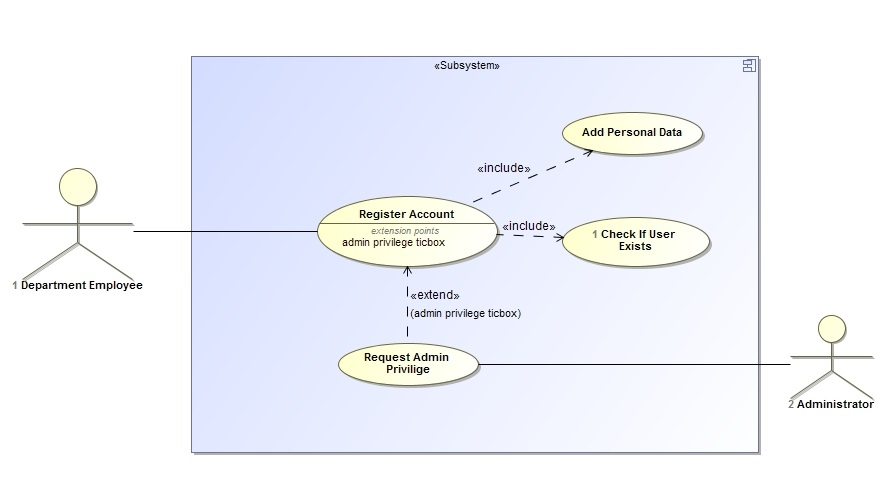
\includegraphics[width=1\textwidth]{./Registration.jpg}\\[1.5cm]
	 
	\subsubsection{Login Use Case Diagram}
	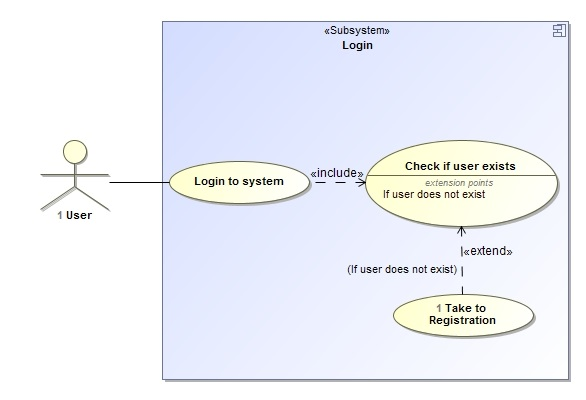
\includegraphics[width=1\textwidth]{./Login.jpg}\\[1.5cm] 
	
	\subsubsection{Logout Use Case Diagram}
	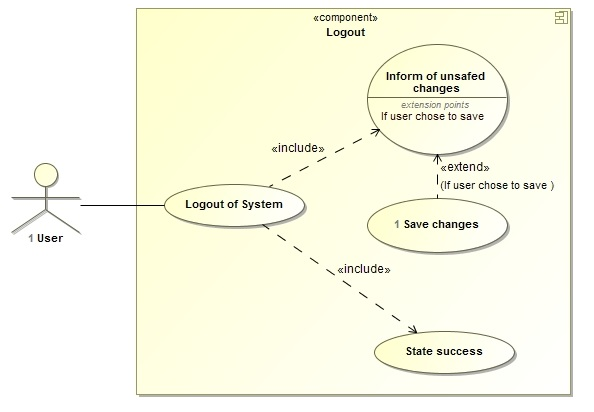
\includegraphics[width=1\textwidth]{./Logout.jpg}\\[1.5cm]
	
	\subsubsection{Create Publication Use Case Diagram}
	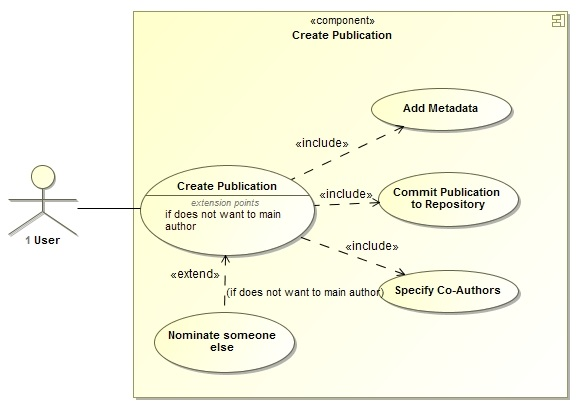
\includegraphics[width=1\textwidth]{./CreatePublication.jpg}\\[1.5cm]

	\subsubsection{Add/Remove Author Use Case Diagram}
	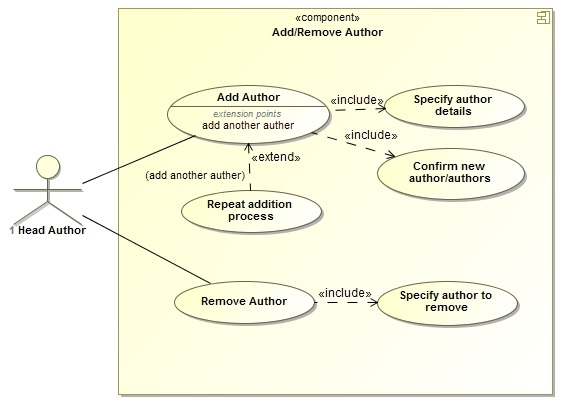
\includegraphics[width=1\textwidth]{./AddRemoveAuthor.jpg}\\[1.5cm]

	\subsubsection{Edit Publication Use Case Diagram}
	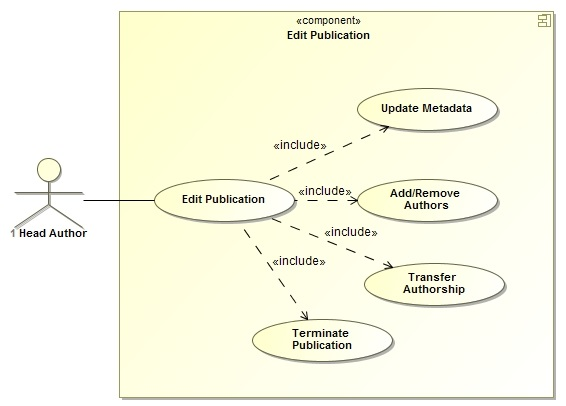
\includegraphics[width=1\textwidth]{./EditPublication.jpg}\\[1.5cm]

	\subsubsection{View Publication Use Case Diagram}
	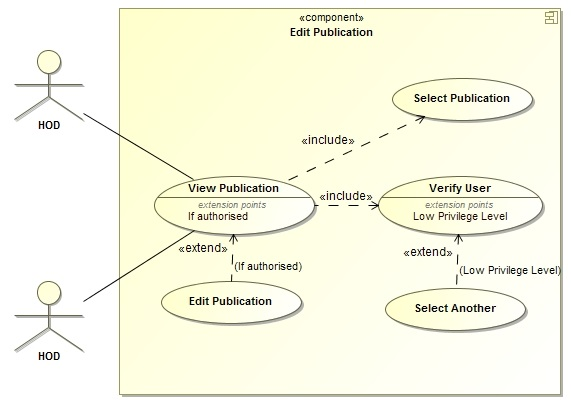
\includegraphics[width=1\textwidth]{./ViewPublication.jpg}\\[1.5cm]
	
	\subsubsection{View Profile Use Case Diagram}
	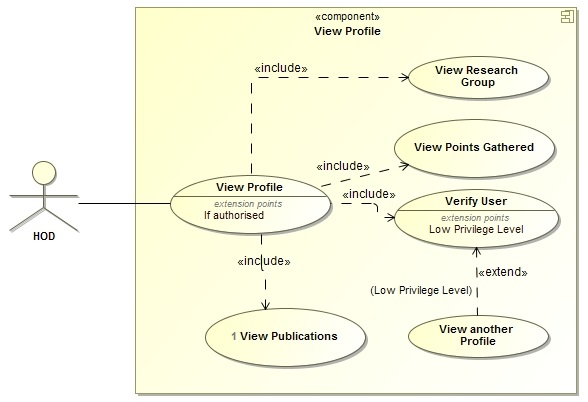
\includegraphics[width=1\textwidth]{./ViewProfile.jpg}\\[1.5cm]
	
	\subsubsection{Edit Profile Use Case Diagram}
	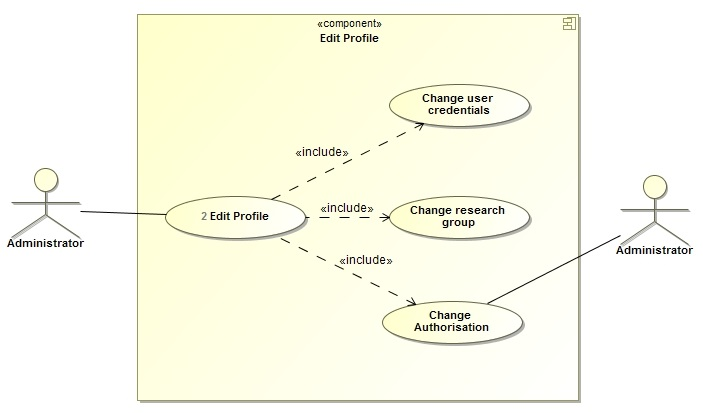
\includegraphics[width=1\textwidth]{./EditProfile.jpg}\\[1.5cm]
	
	\subsubsection{Generate Report Use Case Diagram}
	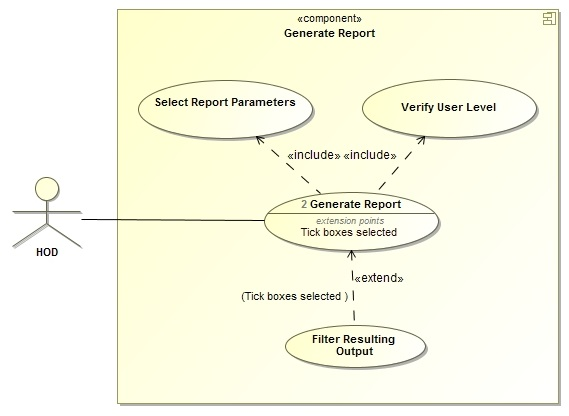
\includegraphics[width=1\textwidth]{./GenerateReport.jpg}\\[1.5cm]
		
\subsection{Process specifications}
	\subsubsection{Registration Activity Diagram}
	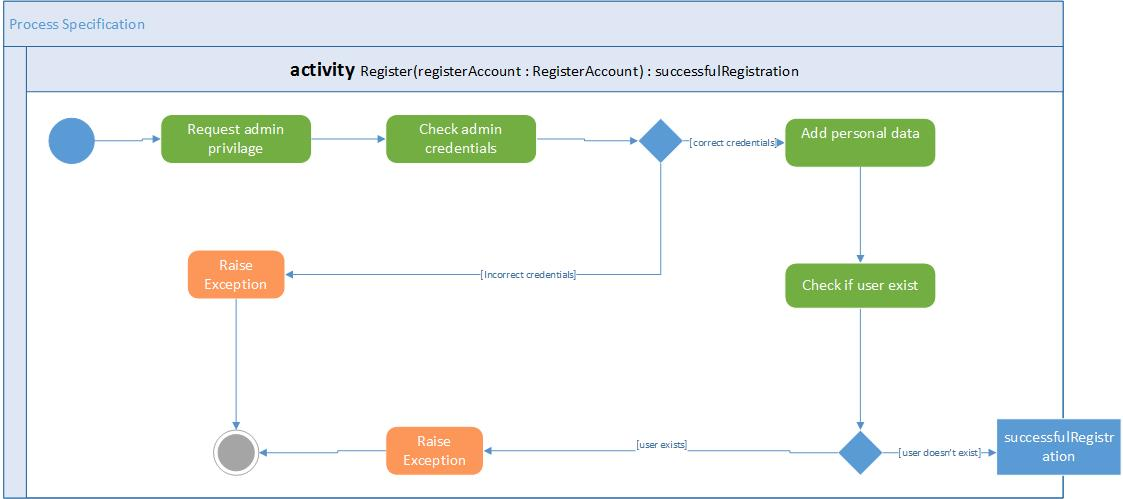
\includegraphics[width=1\textwidth]{./Activity_Register.jpg}\\[1.5cm]
	 
	\subsubsection{Login Activity Diagram}
	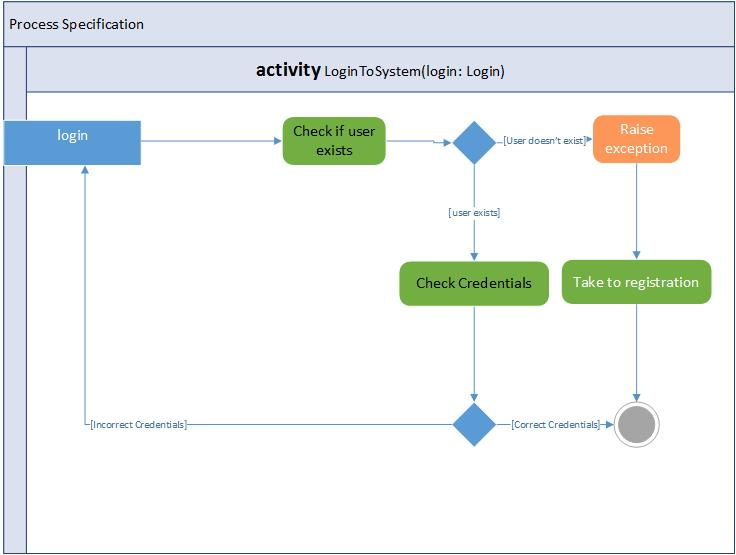
\includegraphics[width=1\textwidth]{./activity_login.jpg}\\[1.5cm] 
	
	\subsubsection{Logout Activity Diagram}
	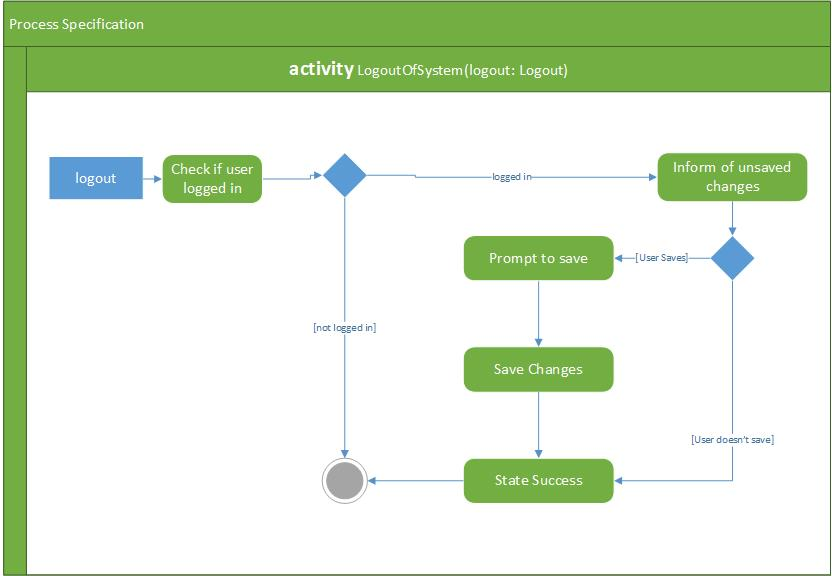
\includegraphics[width=1\textwidth]{./activity_logout.jpg}\\[1.5cm]
	
	\subsubsection{Create Publication Activity Diagram}
	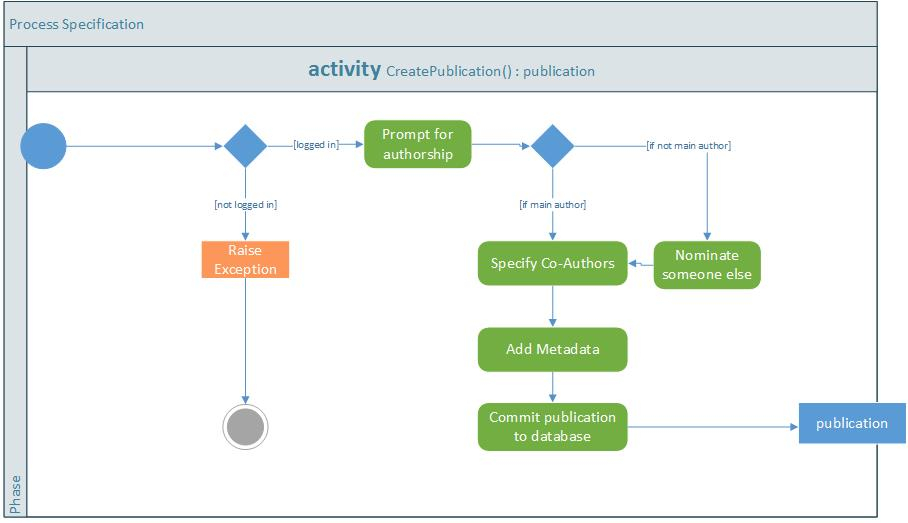
\includegraphics[width=1\textwidth]{./activity_create_pub.jpg}\\[1.5cm]

	\subsubsection{Remove Author Activity Diagram}
	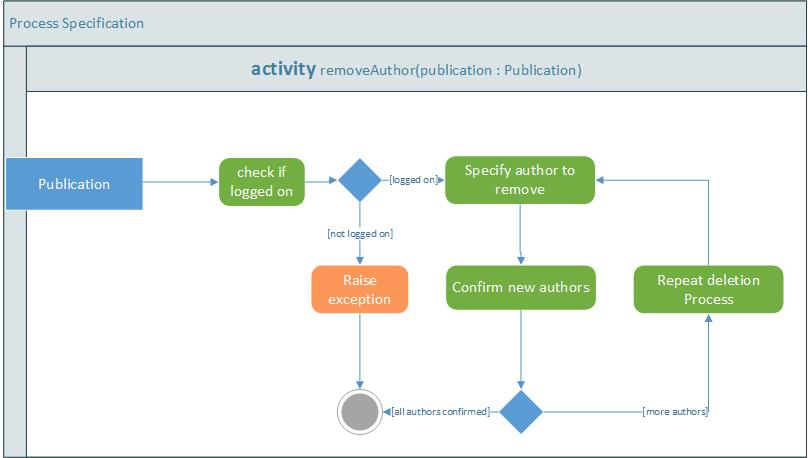
\includegraphics[width=1\textwidth]{./activity_remove_author.jpg}\\[1.5cm]

	\subsubsection{Add Author Activity Diagram}
	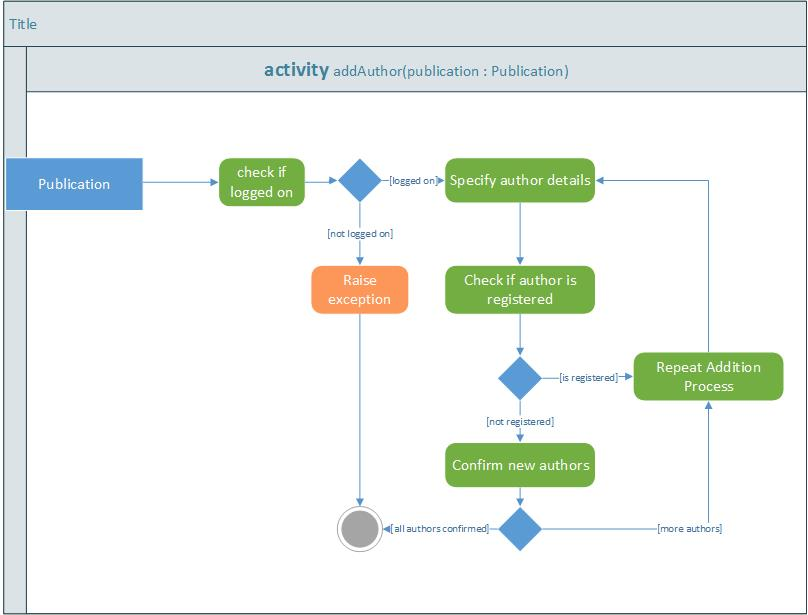
\includegraphics[width=1\textwidth]{./activity_add_author.jpg}\\[1.5cm]

	\subsubsection{Edit Publication Activity Diagram}
	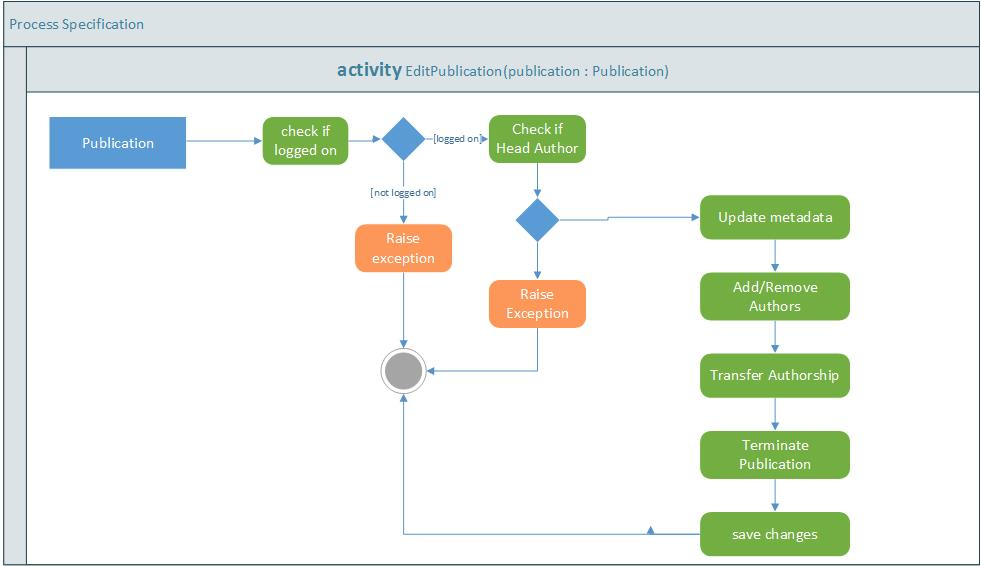
\includegraphics[width=1\textwidth]{./activity_edit_pub.jpg}\\[1.5cm]

	\subsubsection{View Publication Activity Diagram}
	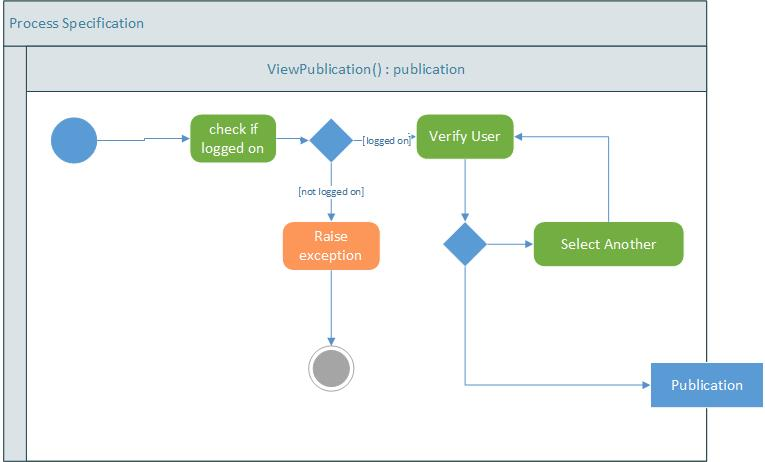
\includegraphics[width=1\textwidth]{./activity_view_pub.jpg}\\[1.5cm]
	
	\subsubsection{View Profile Activity Diagram}
	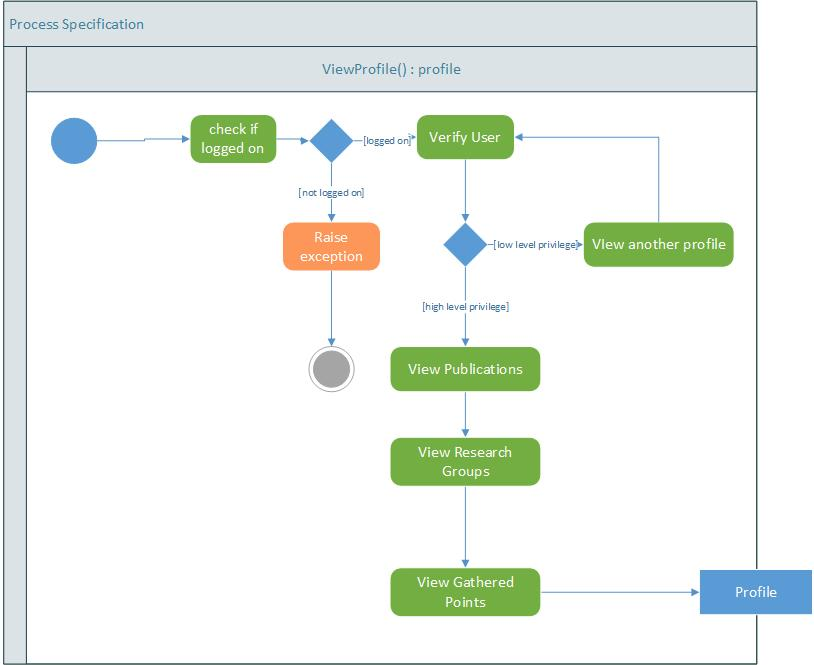
\includegraphics[width=1\textwidth]{./actvity_view_profile.jpg}\\[1.5cm]
	
	\subsubsection{Edit Profile Activity  Diagram}
	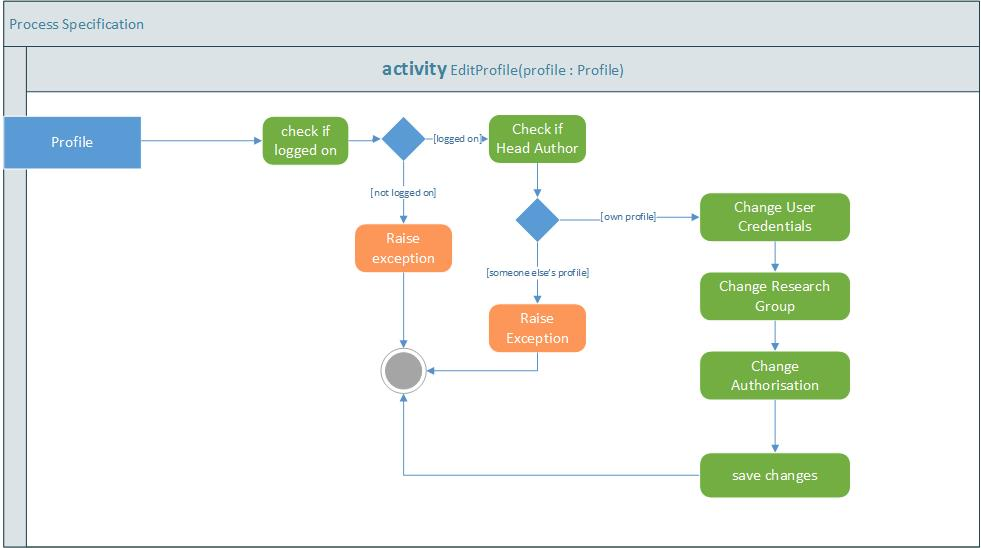
\includegraphics[width=1\textwidth]{./activity_edit_profile.jpg}\\[1.5cm]
	
	\subsubsection{Generate Report Activity Diagram}
	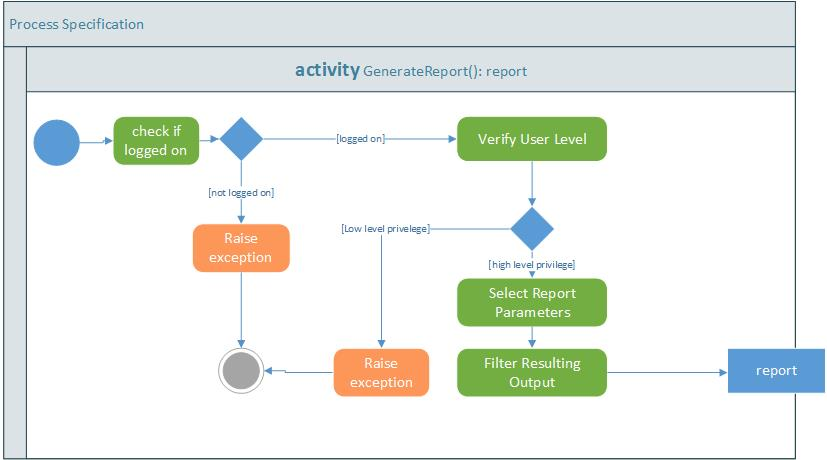
\includegraphics[width=1\textwidth]{./activity_generate_report.jpg}\\[1.5cm]

\subsection{Domain Model}
	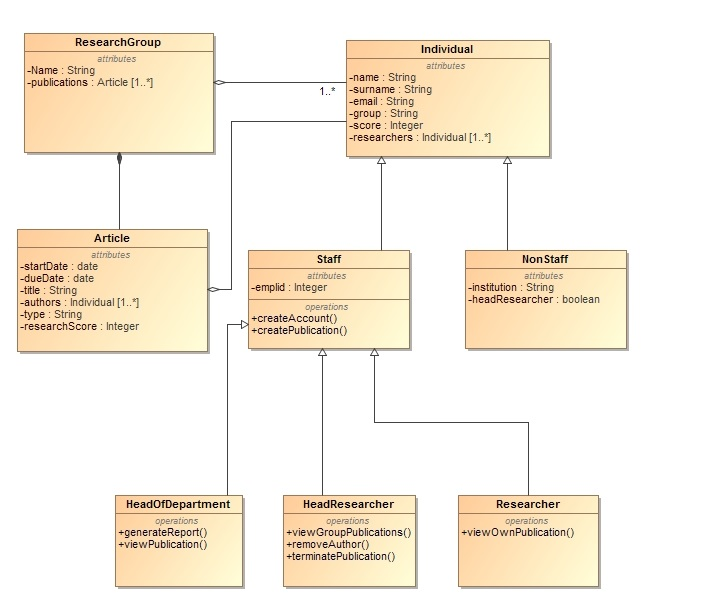
\includegraphics[width=1\textwidth]{./Domain.jpg}\\[1.5cm]
\newpage
\section{Open Issues}
As clarification, the client does not want to store any of the research articles on the system. They only want a link to where the research is being worked on.

The client has expressed an interest in a notification functionality, but has said that one is not nessassary.
\end{document}
